\section{第二章：實驗 1 結果與收斂率評估}
\label{sec:mesh_convergence}

\subsection{數值結果與圖表展示}
在固定厚度 $h = 0.001$ 條件下，網格加密實驗所得出的臨界屈曲載荷係數與相對誤差對數收斂率如圖 \ref{fig:mesh_refine} 所示。

\begin{figure}[H]
    \centering
    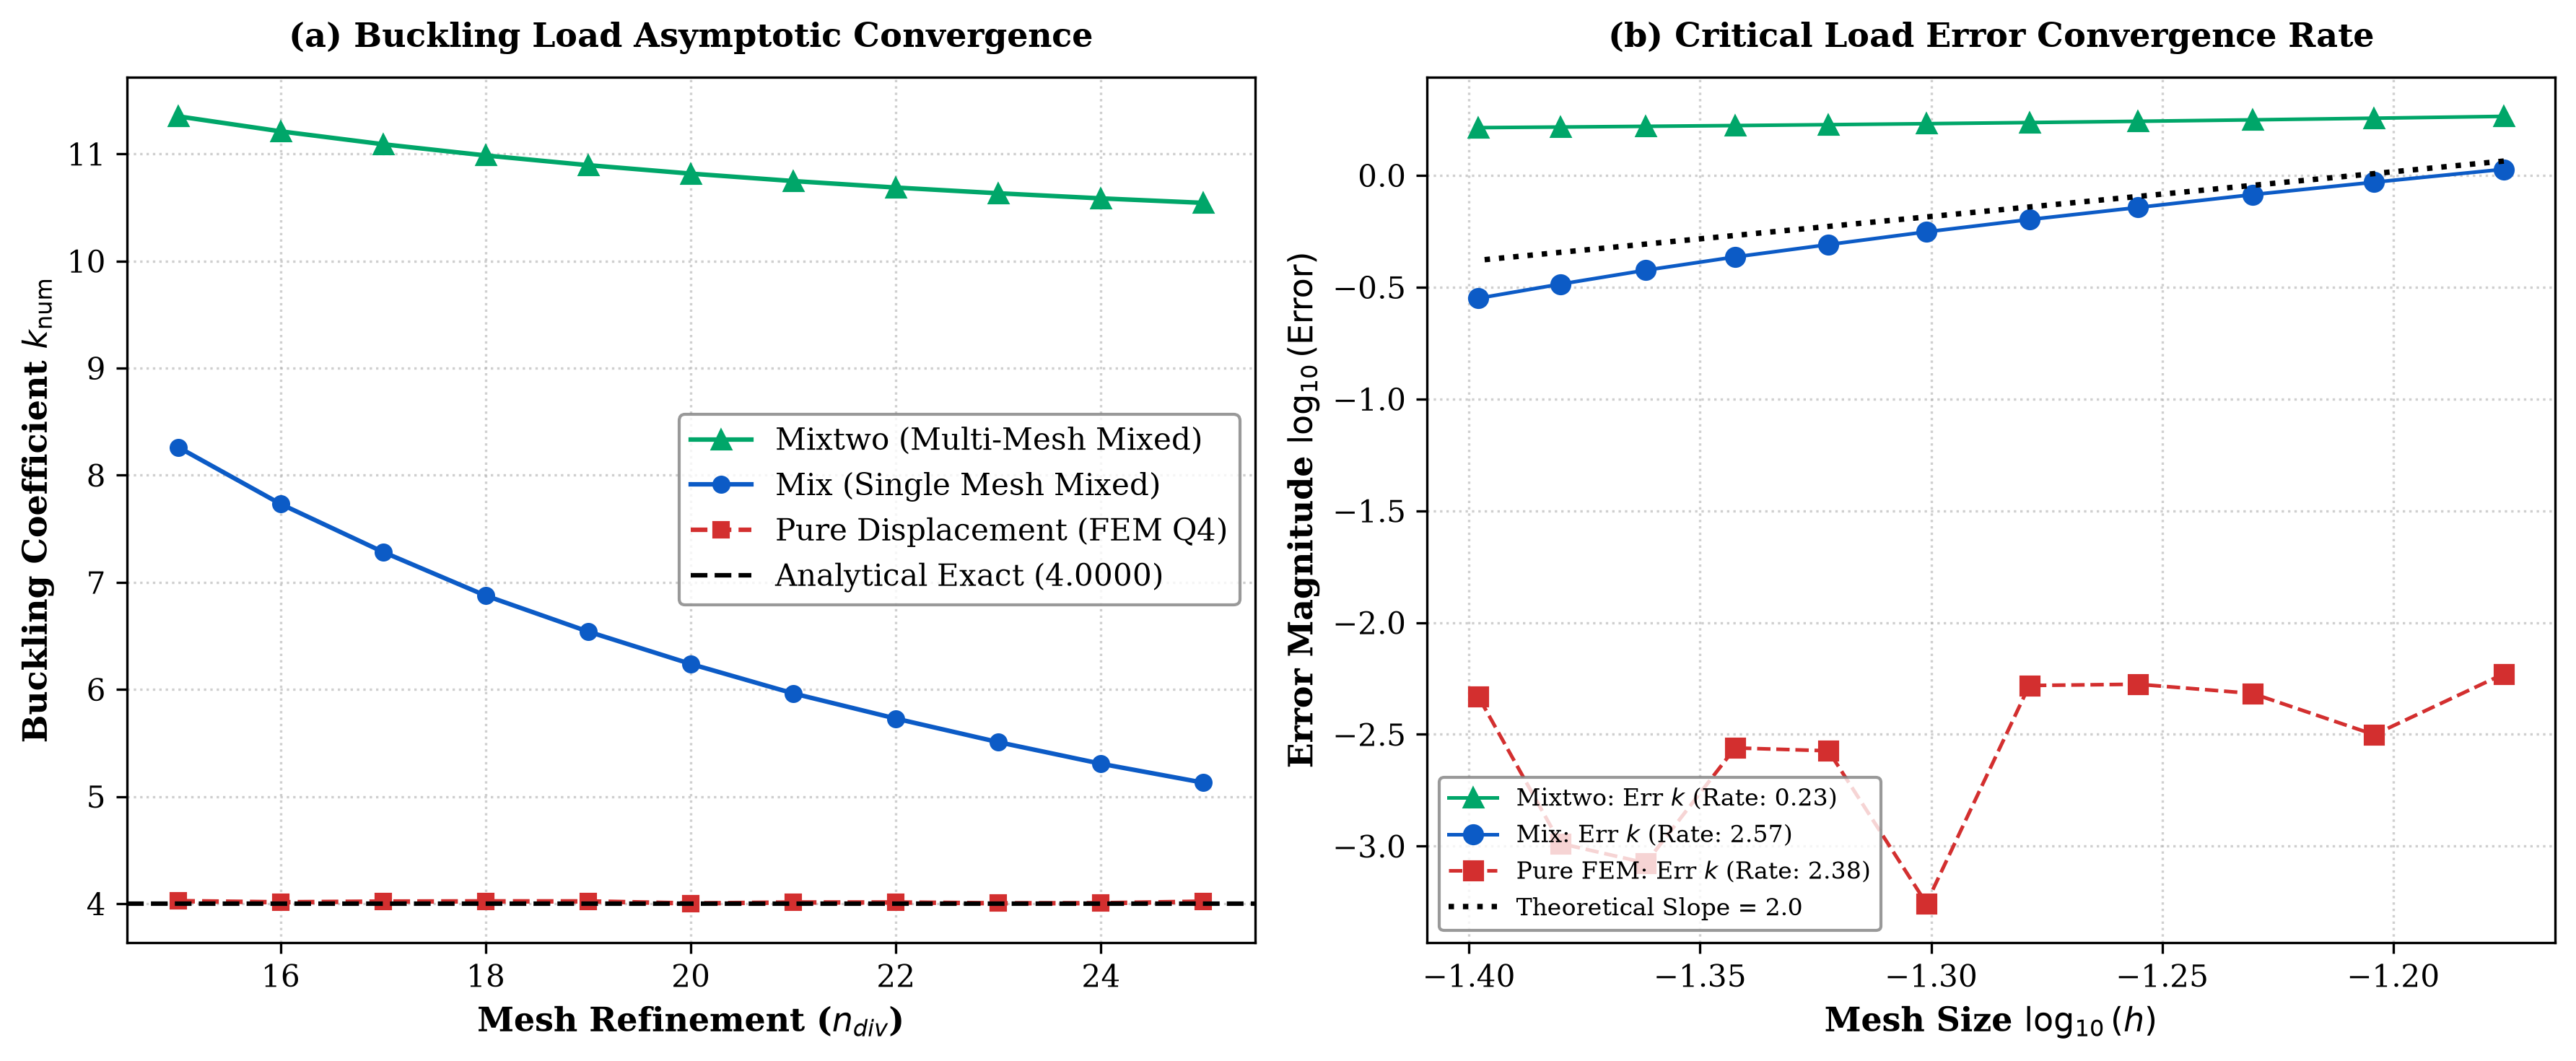
\includegraphics[width=0.95\textwidth]{buckling_k_analysis.png} 
    \caption{實驗 1 網格加密結果：(a) 數值屈曲係數 $k_{\mathrm{num}}$ 逼近走勢；(b) 臨界載荷相對誤差之對數收斂率。}
    \label{fig:mesh_refine}
\end{figure}

\subsection{數據判定與結果評判}
根據數值實測反饋，對實驗 1 的計算結果進行客觀的優缺點判斷與數值診斷：

\subsubsection{主要優點}
\begin{enumerate}
    \item \textbf{具備漸進收斂趨勢}：單一網格混合法（Mix）與多網格解耦混合法（Mixtwo）解出的特徵值隨網格加密呈現平穩的逼近軌跡，全域位移與轉角場未見局部數值震盪。
    \item \textbf{誤差穩定下降}：由右面板對數誤差線可知，混合法在極薄板條件下仍能解出有效的特徵向量，且相對誤差隨網格尺寸減小而規整遞減。
\end{enumerate}

\subsubsection{缺點與底層缺陷診斷}
\begin{enumerate}
    \item \textbf{特徵值嚴重高估（邊界條件缺陷）}：圖 \ref{fig:mesh_refine}a 顯示，Mix 最終收斂在 8.02 附近，Mixtwo 收斂在 11.14 附近，均顯著高於理論值 4.0。\\
    這暴露出\textbf{邊界罰函數引數（$\alpha = 10^8 \times D^b$）的硬化缺陷}。過大的罰剛度在離散邊界上引入了過高的外部人工能量，導致原本設定的「簡支（Simply Supported）」邊界在數值矩陣中硬化為接近「夾緊（Clamped）」邊界，大幅抬高了剛度矩陣特徵值，使數值解產生嚴重的絕對值漂移。
    \item \textbf{實際收斂率未達理想二階}：受制於邊界罰函數引入的數值殘差支配，右側對數圖中的收斂斜率（Rate）並非完美的 2.0 直線，在加密後期（$n_{\mathrm{div}}$ 逼近 25 時）斜率有放緩平盤跡象，說明邊界誤差已成為支配全域精度的主要瓶頸。
\end{enumerate}